\section{Results}
\subsection{Datasets}
%\begin{figure}
%	\centering
%	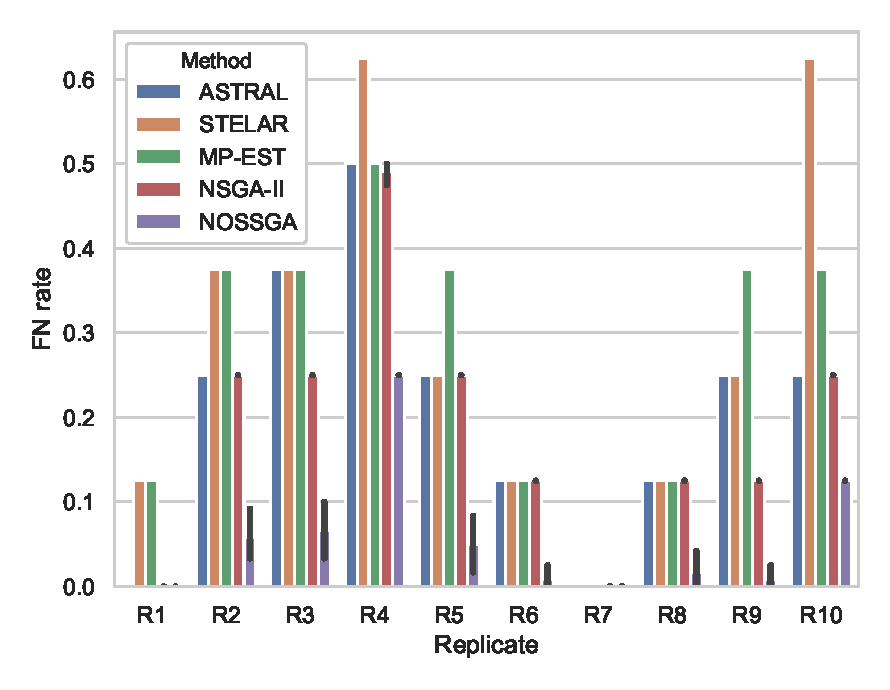
\includegraphics[width=0.6\textwidth]{Figure/10-taxon_10_replicates}
%	\caption{10-taxon.} \label{fig1}
%\end{figure}
%\begin{figure}
%	\centering
%	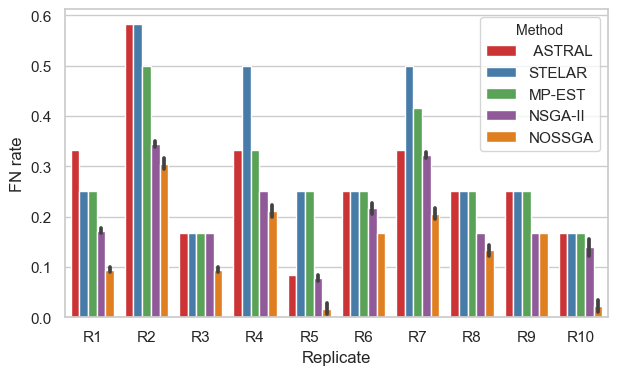
\includegraphics[width=0.6\textwidth]{Figure/15-taxon_10_replicates}
%	\caption{15-taxon.} \label{fig2}
%\end{figure}
\begin{figure}[!htbp]
	\centering
	\begin{adjustwidth}{-4.5cm}{}
	\begin{subfigure}[b]{0.5\textwidth}
		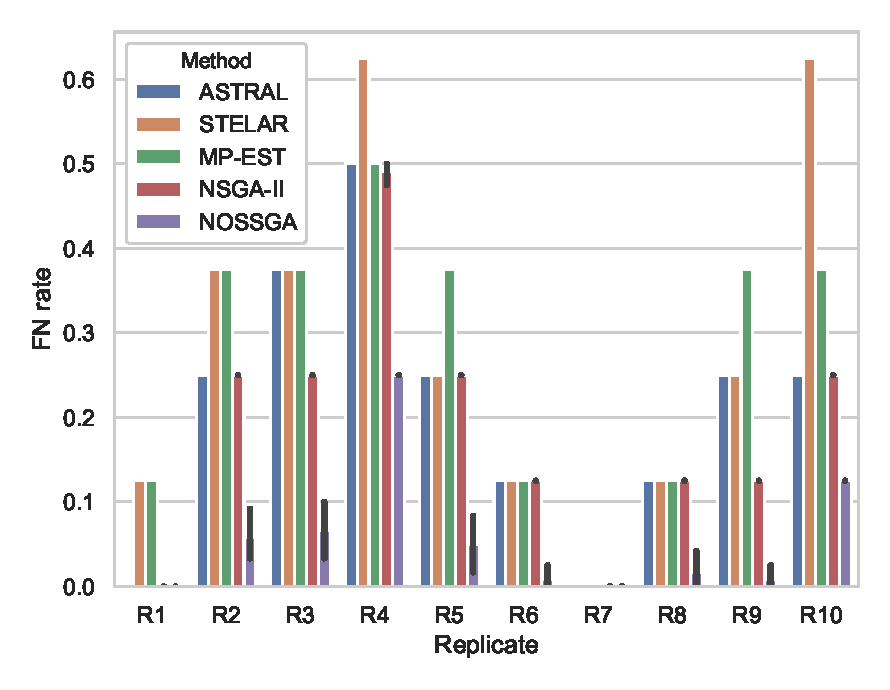
\includegraphics[width=\textwidth]{Figure/10-taxon_10_replicates}
		\caption{10-taxon}
		%\label{fig:con_pr06}
	\end{subfigure}%
	\begin{subfigure}[b]{0.5\textwidth}
		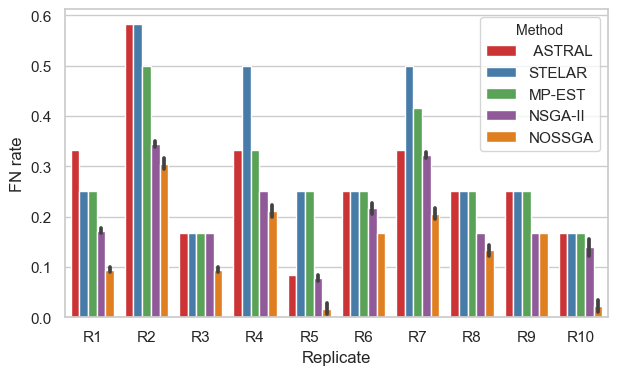
\includegraphics[width=\textwidth]{Figure/15-taxon_10_replicates}
		\caption{11-taxon}
		%\label{fig:con_pr07}
	\end{subfigure}%
	\begin{subfigure}[b]{0.5\textwidth}
		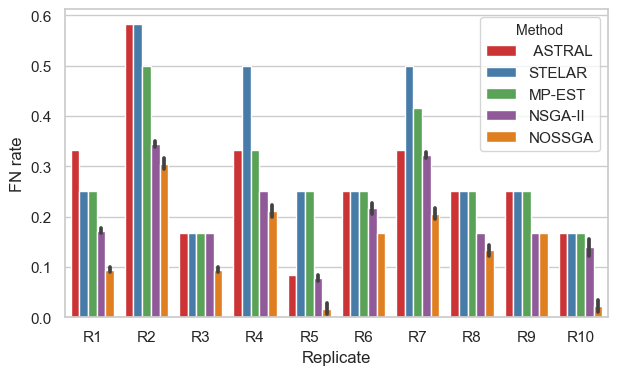
\includegraphics[width=\textwidth]{Figure/15-taxon_10_replicates}
		\caption{15-taxon}
		%\label{fig:con_pr09}
	\end{subfigure}%
	\end{adjustwidth}
	\caption{Comparison of ASTRAL, MP-EST, STELAR, NSGA-II and NOSSGA on 10 replicates of 3 datasets.}
	\label{fig:datasets}

\end{figure}
\subsection{Results on 10-taxon dataset}
\subsection{Results on 11-taxon dataset}
\subsection{Results on 15-taxon dataset}
\subsection{Discussion}